\section{Navigation}\label{sec:navigation}
As mention in the previous Section we use the navigation drawer in our application, the navigation drawer is a navigation design pattern acknowledged and used by Google.\cite{guidelines-navigationdrawer} The navigation drawer is the central view for navigation in our application. It is a powerful design that allows the user from any views in the application to navigate to top level views. The navigation drawer is expanded from the left of the application.
\begin{figure}[H]
\centering
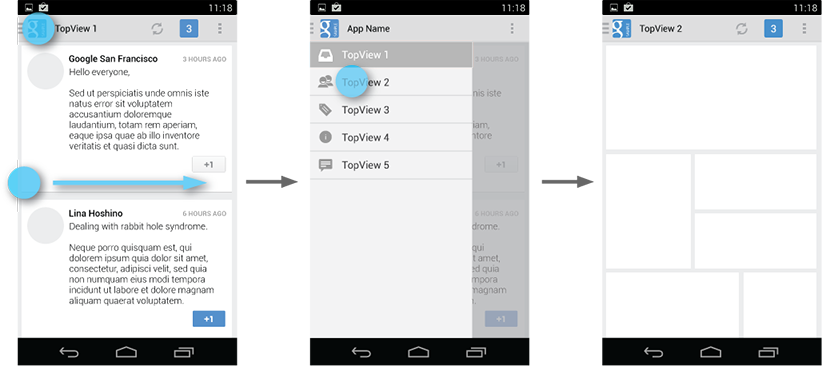
\includegraphics[width=0.9\linewidth]{img/screenshots/navigation_drawer_overview.png}
\caption{Navigation drawer overview \cite{guidelines-navigationdrawer}}
\label{fig:navigationdrawer}
\end{figure}
There are two different ways of expanding the navigation drawer, the consistent one being swiping from the left edge of the screen to the centre, this can always be achieved no matter the context. 
The second one being pressing the button in the top left corner, the button the marked with three lines, \autoref{fig:navigationdrawer} illustrates this. 
The reason for the second option not being consistent is if the user navigates to a lower level view, this will change the button to a return button instead, that if pressed will navigate the user back to the top most view. 
Each item in the navigation drawer navigates to different top-level pages in the application or typical main actions like sign in/sign out.

\subsection{Application navigation}
In our application we plan to implement six top level views ingredient search, recipe search, favourites, shopping list, settings, and sign in/sign out. 
Our application only has one lower level view which is the display of a recipe, it is a lower level view because it is only accessible through other views.
Some views or actions in the application might require the user to be signed in, for them to be available. 
Like the favourites view, which displays the recipes that the user has favourited. 

If the user is not signed in when entering the favourite view, they are met with a text asking them to sign in, this should always happen in the case the user tries to use user-functionalities. 
In the bottom of the navigation drawer we plan to add an item with the action of signing in or signing out the user, it is located in the bottom of the navigation drawer to signalise its difference with the other items in the navigation drawer.
\begin{figure}[H]
\centering
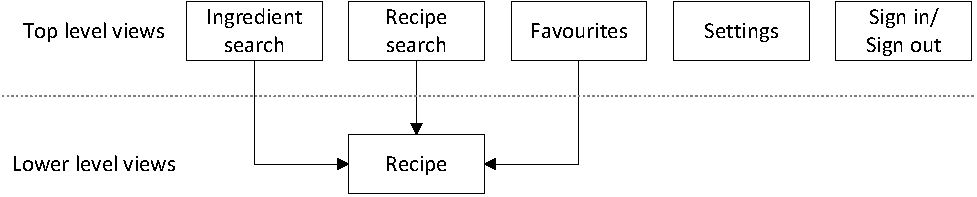
\includegraphics[width=1.0\linewidth]{img/navigation.pdf}
\caption{Navigation view flow}
\label{fig:navigationViews}
\end{figure}
\autoref{fig:navigationViews} shows the views that are accessible in the application, and the navigation flow between the views. 
It can be seen that to reach the recipe view you have to go through ingredient search, recipe search or favourites. It should be noted that it is always possible reach to top level views.
